\documentclass[11pt,a4paper]{article}
\usepackage[margin=26mm,headheight=14pt]{geometry}
\usepackage[T1]{fontenc}
\usepackage{libertinus}
\usepackage{microtype}
\usepackage{amsmath,amsthm,mathtools}
\usepackage{libertinust1math}
\usepackage{aliascnt}
\usepackage{graphicx,booktabs,array,tabularx,longtable}
\usepackage{enumitem}
\usepackage{xcolor}
\usepackage{fancyhdr}
\usepackage{xurl}
\usepackage[hidelinks,pdfauthor={Research manuscript prepared for Vladimir Reshetnikov},
 pdftitle={Sharp Conditioning Laws for Uniform Random Series},
 pdfsubject={Fabius laws, conditional limit theorems, information profiles, and rare-event sampling}]{hyperref}
\usepackage[capitalise,noabbrev]{cleveref}
\usepackage{listings}
\definecolor{ink}{HTML}{203340}
\definecolor{pale}{HTML}{F3F5F6}
\pagestyle{fancy}\fancyhf{}
\fancyhead[L]{\small Sharp conditioning laws for uniform series}
\fancyhead[R]{\small Research manuscript}
\fancyfoot[C]{\thepage}
\setlength{\parskip}{3.5pt}
\setlength{\parindent}{1.2em}
\setlength{\emergencystretch}{2em}
\setcounter{tocdepth}{1}
\numberwithin{equation}{section}
\newtheorem{theorem}{Theorem}[section]
\newaliascnt{lemma}{theorem}
\newtheorem{lemma}[lemma]{Lemma}
\aliascntresetthe{lemma}
\newaliascnt{proposition}{theorem}
\newtheorem{proposition}[proposition]{Proposition}
\aliascntresetthe{proposition}
\newaliascnt{corollary}{theorem}
\newtheorem{corollary}[corollary]{Corollary}
\aliascntresetthe{corollary}
\theoremstyle{definition}
\newaliascnt{definition}{theorem}
\newtheorem{definition}[definition]{Definition}
\aliascntresetthe{definition}
\newaliascnt{question}{theorem}
\newtheorem{question}[question]{Question}
\aliascntresetthe{question}
\theoremstyle{remark}
\newaliascnt{remark}{theorem}
\newtheorem{remark}[remark]{Remark}
\aliascntresetthe{remark}
% ed. (2026-09-30): unnumbered environment for ProveIt editorial notes (no counter is shifted).
\newtheorem*{ednote}{Editorial note (ProveIt, 2026-09-30)}
\newcommand{\N}{\mathbb N}
\newcommand{\R}{\mathbb R}
\newcommand{\E}{\mathbb E}
\newcommand{\Pp}{\mathbb P}
\newcommand{\Qt}{Q_t}
\newcommand{\Pt}{P_t}
\newcommand{\TV}{d_{\mathrm{TV}}}
\newcommand{\KL}{D_{\mathrm{KL}}}
\newcommand{\Exp}{\operatorname{Exp}}
\newcommand{\Var}{\operatorname{Var}}
\newcommand{\Cov}{\operatorname{Cov}}
\newcommand{\Law}{\mathcal L}
\newcommand{\ind}{\mathbf 1}
\newcommand{\phiN}{\varphi}
\newcommand{\PhiN}{\Phi}
\newcommand{\repo}{\texttt{ProveIt}}
\DeclareMathOperator{\supp}{supp}
\DeclareMathOperator{\osc}{osc}
\lstset{basicstyle=\ttfamily\small,columns=fullflexible,keepspaces=true,
 breaklines=true,frame=single,rulecolor=\color{black!25},showstringspaces=false}

\begin{document}
\hypersetup{pageanchor=false}
\begin{titlepage}
\vspace*{8mm}
{\large\sffamily\color{ink} PROVEIT RESEARCH SERIES\par}
\vspace{12mm}
{\Huge\bfseries Sharp Conditioning Laws\par
 for Uniform Random Series\par}
\vspace{7mm}
{\Large Variance thresholds, boundary phases,\par
 Brownian bridges, and rare-event sampling\par}
\vspace{10mm}
{\normalsize Prepared for Vladimir Reshetnikov\par
 28 September 2026\par}
\vspace{12mm}
\begin{abstract}
Let $S=\sum_{k\ge1}w_kU_k$, where the $U_k$ are independent uniform
random variables and the positive weights are summable. What does an
entire configuration look like when $S$ is forced close to zero? We prove
a conditional-law theorem for the moving exponential tilt of this series.
For every positive summable weight sequence, a coordinate block is
asymptotically unaffected by the conditioning in total variation if and
only if it carries a vanishing fraction of the tilted variance. No
monotonicity or regular spacing of the weights is required. For a
limiting variance fraction $\alpha\in(0,1)$, we calculate the exact
nonzero total-variation profile and the relative-entropy limit
$[-\log(1-\alpha)-\alpha]/2$. At fraction one, total variation tends to
one and relative entropy diverges.

For geometric weights, including the classical Fabius distribution,
we identify an infinite, phase-dependent boundary product law, prove a
Brownian-bridge limit for conditioned partial sums, and show that the
rescaled gap to the conditioning boundary becomes an independent
exponential random variable. The same variance criterion applies to
stretched-exponential and polynomial weights. A lazy rejection sampler
is exact in a real-arithmetic model and uses asymptotically
$\sqrt{2\pi}\,n^{3/2}$ scalar uniform draws per accepted geometric
configuration, where $n$ is the effective dimension.

The proofs are given in full. Exact finite-simplex formulas and
reproducible numerical experiments check the constants, but are not
used as substitutes for proofs. The contribution is a conditional
configuration theory connected to the repository's scalar Fabius
endpoint program; neither global priority nor Lean verification is
asserted.
\end{abstract}
\vfill
\noindent\small
\textbf{Scope and status.} Independent research draft, not externally
refereed. Exponential tilting and the Gibbs conditioning principle are
classical. The theorem package below is proved here under its displayed
hypotheses; its precise relationship to the full prior literature remains
a priority-review task. Repository snapshot:
\texttt{e2b1f016a94102663f12b970e6dd434229f90d01}.
\end{titlepage}
\pagenumbering{roman}
\hypersetup{pageanchor=true}
\tableofcontents
\clearpage
\pagenumbering{arabic}

\section{From scalar endpoint probabilities to conditioned configurations}
\label{sec:introduction}

\subsection{The connection with the repository}
The Fabius--Rvachev development in \repo\ contains a substantial
endpoint-asymptotic program. The pinned source
\texttt{PaperFabiusAsymptotic.lean} distinguishes the valid
Laplace-product and saddle-point route from an older invalid residual
argument, and records all-orders exact-phase results and carefully
scoped inverse statements \cite{repo}. The present article starts with
the same probabilistic object but asks a different question: not merely
\emph{how small is the endpoint probability}, but \emph{which
configurations realize that event}.

The original probabilistic construction of Fabius and the later
exposition of Arias de Reyna supply the historical context
\cite{fabius,arias}. In the normalization used here,
\begin{equation}\label{eq:fabius-series}
 S_{1/2}=\sum_{k\ge1}2^{-k}U_k,\qquad
 F(x)=\Pp(S_{1/2}\le x),\qquad U_k\sim\operatorname{Unif}[0,1].
\end{equation}
Thus $F$ is the bounded distribution function on $[0,1]$, not a signed
extension of the Fabius function outside that interval. The general
geometric model is $S_q=\sum q^kU_k$, $0<q<1$.

Four precise research questions organize this article.
\begin{description}[leftmargin=3em,style=nextline]
\item[Q1: Independence threshold.]
How large can a collection of coordinates be before the constraint
$S\le x$ changes its product-tilted law by a nonvanishing amount?
\item[Q2: The price of a macroscopic block.]
When that change does not vanish, can one calculate its exact
information-theoretic size, rather than only an upper bound?
\item[Q3: Bulk and boundary geometry.]
What are the fluctuation process, the distance to the constraint, and
the transition between strongly tilted and almost untouched coordinates?
\item[Q4: Constructive realization.]
Can one sample the conditioned law without waiting for an event whose
original probability is extremely small?
\end{description}
These are questions formulated here from the repository's endpoint
program. We do not identify them with a named published conjecture, or
claim that a keyword search establishes their absence from every
repository manuscript.

\subsection{Prior work and the novelty boundary}
Conditional approximation by exponential families is classical.
Diaconis and Freedman developed conditional limit theorems and finite
forms of de Finetti's theorem \cite{diaconisfreedman}; Dembo and Zeitouni
explicitly considered growing blocks and sharp Gibbs-conditioning
bounds \cite{dembozeitouni}. Consequently, the assertion that small
blocks approach a tilted product law is \emph{not} presented as a new
principle.

A recent comparison point is Cator and Ferrari's Gibbs principle for
independent, not necessarily identically distributed, log-concave
integer-valued variables \cite{catorferrari}. Their setup uses a fixed
tilt and a growing finite sum, with a no-condensation condition. Here
we work with a continuous infinite weighted series, let the tilt tend
to infinity, and compute marginal total-variation and entropy profiles
for an arbitrary deterministic subset of coordinates. Our proofs do
not invoke their theorem. Their result is important context, not a
missing lemma being silently assumed.

The substantive development below is the combination of an explicit
variance-fraction theorem for every positive summable weight sequence,
its complete endpoint dichotomy, an
infinite geometric boundary law, a joint bridge--slack limit, and a
proved lazy-sampling cost. The Gaussian profile itself is naturally
related to classical ensemble equivalence and already appears in a
finite-simplex calculation. What is established here is its validity
for the specified moving-tilt random-series problem, with the
hypotheses and consequences made explicit. The removal of weight
regularity is obtained by using log-concavity to upgrade a central
limit theorem to uniform density convergence. A targeted literature
check is not a certification of worldwide novelty.

\subsection{Conventions}
All random coordinates are indexed by $\N=\{1,2,\ldots\}$. All
logarithms are natural. For probability measures $P,Q$ on the same
measurable space,
\[
 \TV(P,Q)=\sup_A|P(A)-Q(A)|
          =\frac12\int|dP-dQ|,
 \qquad
 \KL(P\Vert Q)=\int\log\frac{dP}{dQ}\,dP,
\]
with relative entropy $+\infty$ when absolute continuity fails. The
standard normal density and distribution function are $\phiN$ and
$\PhiN$. An exponential random variable has rate one unless stated
otherwise. The notation $o(1)$ always refers to $t\to\infty$, except
where a different limiting variable is specified.

\section{The variance-fraction theorem}
\label{sec:main}
Let $w_k>0$ and $\sum_kw_k<\infty$. On the product uniform probability
space $(\Omega,P)$ define
\[
 S=\sum_{k\ge1}w_kU_k,\qquad
 L(t)=\E_P e^{-tS},\qquad
 \frac{d\Qt}{dP}=\frac{e^{-tS}}{L(t)},\quad t>0.
\]
Set $a_k=tw_k$ and introduce the functions
\begin{equation}\label{eq:mu-v}
 \mu(a)=1-\frac{a}{e^a-1},\qquad
 v(a)=1-\frac{a^2e^a}{(e^a-1)^2},\qquad a>0.
\end{equation}
The tilted coordinates $Y_k=a_kU_k$ are independent; their means and
variances are $\mu(a_k)$ and $v(a_k)$. Define
\begin{equation}\label{eq:mVx}
 m=m(t)=\sum_k\mu(a_k),\qquad
 V=V(t)=\sum_kv(a_k),\qquad
 x=x(t)=\frac{m(t)}t.
\end{equation}
Finally let
\begin{equation}\label{eq:conditional}
 \Pt=P(\,\cdot\mid S\le x(t)),\qquad
 D_t=t(x(t)-S)\quad\hbox{under }\Pt.
\end{equation}
The map $t\mapsto x(t)$ parametrizes every sufficiently small positive
endpoint; this is proved in \cref{prop:tilt}.

No monotonicity, regular variation, geometric structure, or
nonconcentration hypothesis is imposed on the weights. Summability
and positivity are enough. The local density theorem that makes this
possible is proved in \cref{sec:lclt}.

For a deterministic subset $I=I_t\subseteq\N$, possibly infinite, put
\[
 V_I=\sum_{k\in I}v(a_k),\quad \alpha_t=V_I/V,
 \quad P_{t,I}=\Law_{\Pt}((U_k)_{k\in I}),
 \quad Q_{t,I}=\Law_{\Qt}((U_k)_{k\in I}).
\]
There is no requirement that $I_t$ be an initial segment, nested, or
chosen by a fixed rule independent of $t$. It must not depend on the
realized random coordinates.

\begin{theorem}[Sharp variance threshold and information profiles]
\label{thm:main}
For every positive summable weight sequence, if $\alpha_t\to\alpha\in[0,1)$, then
\begin{align}
 \TV(P_{t,I},Q_{t,I})&\longrightarrow\Delta(\alpha),\label{eq:tv-main}\\
 \KL(P_{t,I}\Vert Q_{t,I})&\longrightarrow
 K(\alpha):=\frac{-\log(1-\alpha)-\alpha}{2}.\label{eq:kl-main}
\end{align}
Here $\Delta(0)=0$, and for $0<\alpha<1$,
\begin{equation}\label{eq:delta}
 \Delta(\alpha)=2\left[\PhiN(d_\alpha)
 -\PhiN\bigl(\sqrt{1-\alpha}\,d_\alpha\bigr)\right],
 \qquad d_\alpha=\sqrt{\frac{-\log(1-\alpha)}{\alpha}}.
\end{equation}
Moreover,
\begin{equation}\label{eq:slack-factor}
 \TV\left(\Law_{\Pt}((U_k)_{k\in I},D_t),
             P_{t,I}\otimes\Exp(1)\right)\longrightarrow0.
\end{equation}
If $\alpha_t\to1$, then total variation tends to $1$ and relative
entropy tends to $+\infty$.

Without assuming that $\alpha_t$ converges, the following three
conditions are equivalent:
\begin{equation}\label{eq:iff}
 V_I=o(V),\qquad
 \TV(P_{t,I},Q_{t,I})\to0,\qquad
 \KL(P_{t,I}\Vert Q_{t,I})\to0.
\end{equation}
\end{theorem}

The quantity governing independence is therefore \emph{variance},
not the number of selected coordinates. In a geometric series most
active coordinates have variance close to one, so count and variance
agree to leading order. For polynomial weights they do not agree
with the same proportionality throughout the active range.

The profile has the endpoint behavior
\begin{equation}\label{eq:profile-ends}
 \Delta(\alpha)\sim\phiN(1)\alpha,\qquad
 K(\alpha)\sim\frac{\alpha^2}{4}\quad(\alpha\downarrow0),
 \qquad \Delta(\alpha)\to1\quad(\alpha\uparrow1).
\end{equation}
For example, a block carrying half the variance has limiting total
variation approximately $0.1660641$ and relative entropy
$0.0965736$ nats. Such a block is not asymptotically independent of
the constraint, even though every fixed collection inside it can
have the usual product limit.

\section{The tilted coordinates and the endpoint parameter}
\label{sec:tilt}

\begin{proposition}[Exact product change of measure]\label{prop:tilt}
For every $t>0$,
\begin{equation}\label{eq:laplace}
 L(t)=\prod_{k\ge1}\frac{1-e^{-tw_k}}{tw_k}>0.
\end{equation}
Under $\Qt$, the coordinates $Y_k=tw_kU_k$ are independent with density
\begin{equation}\label{eq:truncexp}
 h_a(y)=\frac{e^{-y}}{1-e^{-a}}\ind_{[0,a]}(y).
\end{equation}
The sums in \cref{eq:mVx} are finite, $V(t)\to\infty$, and
\[
 x'(t)=-V(t)/t^2<0,\qquad
 x(0+)=\frac12\sum_kw_k,\qquad x(\infty)=0.
\]
In particular $x(t)$ is a continuous bijection from $(0,\infty)$ onto
$(0,\frac12\sum_kw_k)$.
\end{proposition}
\begin{proof}
Since $0\le S\le\sum w_k$, bounded convergence gives the product
formula from finite products. Its positivity also follows immediately
from $e^{-tS}\ge e^{-t\sum w_k}>0$. Factoring the exponential
Radon--Nikodym derivative on every cylinder proves independence and
\cref{eq:truncexp}; cylinder identities determine the countable product
law.

Direct integration by parts shows that the mean and variance of
\cref{eq:truncexp} are
\cref{eq:mu-v}. They satisfy $0<\mu(a)\le a/2$ and $0<v(a)<1$.
The first inequality follows because an exponentially decreasing
weight on $[0,a]$ moves the uniform mean downward. Also
$v(a)\le a^2/4$, the elementary range bound for variance.
Thus $m(t)\le(t/2)\sum w_k$ and
$V(t)\le(t^2/4)\sum w_k^2<\infty$.
For any fixed $M$, $\sum_{k\le M}v(tw_k)\to M$; hence $V(t)\to\infty$.

Differentiation under expectation is valid because $S$ is bounded.
It yields $x(t)=-(\log L)'(t)=\E_{\Qt}S$ and
$x'(t)=-\Var_{\Qt}S=-V(t)/t^2$. The limiting value at zero follows
from dominated convergence. For each fixed $k$, the tilted mean of
$w_kU_k$ is $\mu(tw_k)/t\to0$, and it is bounded by $w_k/2$.
Dominated convergence for the summable series proves the limit at
infinity. Strict monotonicity and continuity finish the proof.
\end{proof}

\begin{lemma}[Uniform moment estimates]\label{lem:moments}
For every real $p\ge2$ there is a finite constant $C_p$ such that,
for $H_a$ of density \cref{eq:truncexp},
\begin{equation}\label{eq:moments}
 \E|H_a-\mu(a)|^p\le C_pv(a),\qquad a>0.
\end{equation}
There are absolute constants $c,C>0$ for which
\[
 c\min(a^2,1)\le v(a)\le C\min(a^2,1),\qquad a>0.
\]
The small-width expansions are
\begin{align}
 \mu(a)&=\frac a2-\frac{a^2}{12}+\frac{a^4}{720}
               -\frac{a^6}{30240}+O(a^8),\label{eq:mu-series}\\
 v(a)&=\frac{a^2}{12}-\frac{a^4}{240}
               +\frac{a^6}{6048}+O(a^8),\label{eq:v-series}
\end{align}
and $v(a)=\mu(a)-a\mu'(a)$.
\end{lemma}
\begin{proof}
The variable $H_a/a$ has density
$a e^{-au}/(1-e^{-a})$ on $[0,1]$, converging uniformly to one as
$a\downarrow0$. Its centered $p$th absolute moment stays bounded,
while its variance tends to $1/12$. Thus the ratio in
\cref{eq:moments} is $O(a^{p-2})$ at zero.
As $a\to\infty$, the densities $h_a$ converge to the exponential
density and, for $a\ge1$, are bounded by
$(1-e^{-1})^{-1}e^{-y}$ on $[0,\infty)$. All relevant moments
converge; in particular $v(a)\to1$. On each remaining compact
interval of positive widths the ratio is continuous with a positive
denominator. These three regions prove the assertions about moments
and variance. Taylor expansion of $a/(e^a-1)$ gives
\cref{eq:mu-series,eq:v-series}; direct differentiation gives the last
identity.
\end{proof}

For a subset $J\subseteq\N$, write
\begin{equation}\label{eq:zJ}
 Z_J=\sum_{k\in J}\bigl(Y_k-\mu(a_k)\bigr),\qquad
 V_J=\Var_{\Qt}(Z_J).
\end{equation}
The sum converges absolutely, since
$\sum|Y_k-\mu(a_k)|\le\sum(a_k+\mu(a_k))<\infty$ for fixed $t$.
This elementary fact avoids any ambiguity about rearranging or
splitting infinitely many coordinates.

\section{A local central limit theorem without weight regularity}
\label{sec:lclt}
The crucial analytic point is a \emph{density} approximation, not
merely a central limit theorem. The conditioning is sensitive to a
window of width one in $Z$, whereas its standard deviation is
$\sqrt V$. A Fourier tail estimate based on many support widths
bounded away from zero would introduce an unnecessary restriction.
Log-concavity removes that restriction entirely.

\subsection{Why every subset sum has a log-concave density}
A nonnegative function $f$ is log-concave if
\[
 f((1-\lambda)x+\lambda y)\ge f(x)^{1-\lambda}f(y)^\lambda
 \quad(0<\lambda<1).
\]
Zeros outside an interval are allowed. The densities $h_a$ in
\cref{eq:truncexp} are log-concave. We include the required
convolution argument, a one-dimensional instance of the classical
Pr\'ekopa--Leindler mechanism \cite{prekopa}.

\begin{lemma}[Convolution and infinite sums]\label{lem:logconcave}
The convolution of two integrable log-concave functions on $\R$
is log-concave. For fixed $t$ and any subset $J$ containing at
least two indices, $Z_J$ has a bounded continuous compactly
supported log-concave density.
\end{lemma}
\begin{proof}
First establish the integral inequality needed for convolution.
Suppose $F,G$ are positive and continuous on the interiors of their
interval supports, have finite positive integrals, and
\[
 H((1-\lambda)x+\lambda y)\ge F(x)^{1-\lambda}G(y)^\lambda.
\]
Normalize $F,G$ to have integral one, rescaling $H$ accordingly.
Let $T$ be the increasing transport matching their distribution
functions. On the interiors, $T$ is continuously differentiable
and $G(T(x))T'(x)=F(x)$. Set $z(x)=(1-\lambda)x+\lambda T(x)$.
Its derivative is positive. Change variables over its image and
use the displayed hypothesis to obtain
\begin{align*}
 \int H(z)\,dz
 &\ge\int F(x)^{1-\lambda}G(T(x))^\lambda
            [(1-\lambda)+\lambda T'(x)]\,dx\\
 &=\int F(x)\left[(1-\lambda)T'(x)^{-\lambda}
                   +\lambda T'(x)^{1-\lambda}\right]dx
 \ge\int F(x)\,dx=1.
\end{align*}
The last inequality is the weighted arithmetic--geometric mean
inequality. Endpoint values have no effect on these integrals;
improper endpoints are handled by increasing limits. Undoing the
normalization proves
$\int H\ge(\int F)^{1-\lambda}(\int G)^\lambda$.

For log-concave $f,g$, fixed $z_0,z_1$, and
$z_\lambda=(1-\lambda)z_0+\lambda z_1$, apply this inequality to
\[
 F(x)=f(x)g(z_0-x),\quad G(y)=f(y)g(z_1-y),\quad
 H(u)=f(u)g(z_\lambda-u).
\]
Log-concavity of $f$ and $g$ verifies the hypothesis. A nonzero
integrable log-concave function is positive and continuous on the
interior of its interval support, so the preceding proof applies.
If an integral vanishes, the desired convolution inequality is
trivial. This establishes the convolution assertion in the case
needed here and, with the usual immaterial endpoint choices, in
general.

For $Z_J$, finite convolution now proves log-concavity. The
convolution of the first two chosen bounded interval densities is
continuous, bounded, and compactly supported; call it $g$. If $J$
is infinite, convolve $g$ with the law of the remaining partial
sum. Those partial-sum densities converge uniformly to the full
sum density: the omitted uncentered tail is bounded by the sum
of its widths, which tends to zero, and $g$ is uniformly
continuous. More precisely, their supremum difference is at most
the modulus of continuity of $g$ evaluated at that tail bound.
The uniform limit is continuous and log-concave. Its support stays
inside an interval of length $\sum_{k\in J}a_k<\infty$.
Centering is an affine translation and preserves all these
properties.
\end{proof}

\subsection{A shape-based upgrade from weak to uniform convergence}
\begin{lemma}[Log-concave convergence to a Gaussian]\label{lem:shape}
Let $f_j$ be continuous compactly supported log-concave probability
densities on $\R$. If their laws converge weakly to $N(0,1)$, then
\begin{equation}\label{eq:shape}
 \sup_x|f_j(x)-\phiN(x)|\longrightarrow0.
\end{equation}
\end{lemma}
\begin{proof}
Choose a mode $b_j$ of each $f_j$, which exists by compactness.
Log-concavity implies that $f_j$ is nondecreasing to the left of
$b_j$ and nonincreasing to its right. We first prove $b_j\to0$.
If a subsequence had $b_j\ge\varepsilon>0$, its densities would be
nondecreasing on $(0,\varepsilon)$. Two disjoint, ordered intervals
of the same length inside that interval would then have right-hand
mass at least left-hand mass. Weak convergence passes this
inequality to the Gaussian, whose density is strictly decreasing
there, a contradiction. A subsequence with $b_j\le-\varepsilon$
is ruled out on the negative side in the same way.

Let $F_j$ be the distribution functions. Weak convergence to a
continuous distribution implies uniform convergence
$F_j\to\PhiN$: a finite grid controls the compact part by
monotonicity, and two endpoint tail bounds control the rest.
For $x$ in a compact interval bounded away from zero on the
positive side, and a sufficiently small fixed $h>0$, eventual
monotonicity gives
\[
 \frac{F_j(x+h)-F_j(x)}h\le f_j(x)
 \le\frac{F_j(x)-F_j(x-h)}h.
\]
Uniform convergence of the distribution functions followed by
$h\downarrow0$ proves uniform density convergence on that compact
interval. The negative side is identical with reversed
inequalities.

It remains to control the peak. Fix $\delta>0$. Eventually
$|b_j|<\delta/2$, and log-concavity at the midpoint $\delta$ of
$b_j$ and $2\delta-b_j$ gives
\[
 f_j(b_j)\le\frac{f_j(\delta)^2}{f_j(2\delta-b_j)}.
\]
The denominator is positive eventually, by the convergence already
proved away from zero. Hence
\[
 \limsup_j\|f_j\|_\infty
 \le\frac{\phiN(\delta)^2}{\phiN(2\delta)}
 =\phiN(0)e^{\delta^2}.
\]
Let $\delta\downarrow0$ to get the upper bound $\phiN(0)$.
On $[-\delta,\delta]$, unimodality and log-concavity give
$f_j(x)\ge\min(f_j(-\delta),f_j(\delta))\to\phiN(\delta)$.
Together with the peak bound, this proves uniform convergence
through zero, by then letting $\delta\downarrow0$.

Finally, for fixed large $R$, eventual unimodality implies
$\sup_{x\ge R}f_j(x)\le f_j(R)\to\phiN(R)$, and similarly on
$x\le-R$. Let $R\to\infty$. The two tails vanish uniformly,
proving \cref{eq:shape} on the whole real line.
\end{proof}

\begin{theorem}[Unrestricted subset local central limit theorem]
\label{thm:lclt}
Let the weights be any positive summable sequence, and let
$J=J_t$ be any deterministic subset with $V_J(t)\to\infty$.
Then $Z_J$ has a bounded continuous density $f_{t,J}$ for all
sufficiently large $t$, and
\begin{equation}\label{eq:lclt}
 \sup_{z\in\R}\left|
 \sqrt{V_J}\,f_{t,J}(z)-\phiN(z/\sqrt{V_J})\right|\longrightarrow0.
\end{equation}
In particular $\|f_{t,J}\|_\infty\le C/\sqrt{V_J}$ eventually,
and $Z_J/\sqrt{V_J}\Rightarrow N(0,1)$.
\end{theorem}
\begin{proof}
Put $s=\sqrt{V_J}$. The centered third-moment estimate gives
\[
 \frac{\sum_{k\in J}\E|Y_k-\mu(a_k)|^3}{s^3}
 \le\frac{C_3}{s}\longrightarrow0.
\]
Thus the normalized centered sum converges weakly to the standard
Gaussian. Here is a direct characteristic-function justification
also valid for a countably infinite row. For each fixed $u$, expand
the centered factors at $u/s$. Their quadratic terms sum to
$-u^2/2$ and their cubic remainders have total absolute value at
most $C|u|^3/s$. Since $v(a_k)\le1$, the sum of the errors in
replacing each factor by its logarithm is $O(u^4/s^2)$.
Taking the exponential yields convergence of the product to
$e^{-u^2/2}$. The same bounds justify the passage from finite to
countable products, because all moment sums converge for each
fixed $t$.

Since $V_J\to\infty$ and each individual variance is at most one,
$J$ eventually contains at least two indices. By
\cref{lem:logconcave}, the normalized sum has a continuous
compactly supported log-concave density. Apply \cref{lem:shape}
along an arbitrary sequence $t\to\infty$ to obtain
\cref{eq:lclt}. The sequential criterion for a limit then gives
the assertion as stated. Its density bound follows immediately.
\end{proof}

\begin{remark}[The regularity issue is resolved, not assumed away]
An ordinary central limit theorem does not generally imply a
local one. Here it does after using the preserved log-concave
shape. In particular, a plateau of many very narrow coordinates,
an irregular sequence of widely separated scales, or a
nonmonotone ordering of the weights does not require a separate
smoothing assumption. This is why the main theorem applies to
\emph{every} positive summable weight sequence.
\end{remark}

\section{The boundary layer and the information cost of the full law}
\label{sec:slack}
Write $Z=Z_{\N}=tS-m$. The exact change of measure gives
\begin{equation}\label{eq:RN-full}
 \frac{d\Pt}{d\Qt}=\frac{e^Z\ind_{Z\le0}}{J(t)},\qquad
 J(t)=\E_{\Qt}[e^Z\ind_{Z\le0}].
\end{equation}
The quantity $J$ is both a saddle normalization and the eventual
acceptance probability of our sampler.

\begin{theorem}[Saddle normalization and exponential slack]
\label{thm:slack}
For every positive summable weight sequence,
\begin{align}
 J(t)&\sim\frac1{\sqrt{2\pi V(t)}},\label{eq:J}\\
 P(S\le x(t))&\sim\frac{L(t)e^{m(t)}}{\sqrt{2\pi V(t)}}.\label{eq:saddle}
\end{align}
Under $\Pt$, $D_t=-Z$ converges to $\Exp(1)$ in total variation.
For every fixed real $r\ge0$,
\begin{equation}\label{eq:slack-moments}
 \E_{\Pt}D_t^r\longrightarrow\Gamma(r+1).
\end{equation}
\end{theorem}
\begin{proof}
Let $f_t=f_{t,\N}$. By \cref{thm:lclt},
\begin{equation}\label{eq:J-integral}
 J(t)=\int_0^\infty e^{-d}f_t(-d)\,dd.
\end{equation}
For fixed $d$, $\sqrt V f_t(-d)\to\phiN(0)$, and
$\sqrt V f_t(-d)\le C$ uniformly. Dominated convergence gives
\cref{eq:J}. \Cref{eq:RN-full} then yields the exact
identity $P(S\le x)=L(t)e^mJ(t)$, proving \cref{eq:saddle}.

The slack density is
\begin{equation}\label{eq:slack-density}
 p_{D,t}(d)=\frac{e^{-d}f_t(-d)}{J(t)}\ind_{[0,\infty)}(d).
\end{equation}
It tends pointwise to $e^{-d}$ and is bounded by $Ce^{-d}$ for all
large $t$. Dominated convergence proves both its $L^1$ convergence
and \cref{eq:slack-moments}.
\end{proof}

\begin{corollary}[Information and overlap of the full configurations]
\label{cor:full-info}
For every positive summable weight sequence,
\begin{equation}\label{eq:full-kl}
 \KL(\Pt\Vert\Qt)=\frac12\log(2\pi V)-1+o(1),
\end{equation}
and
\begin{equation}\label{eq:overlap}
 1-\TV(\Pt,\Qt)
 \sim\frac{\log V}{2\sqrt{2\pi V}}.
\end{equation}
\end{corollary}
\begin{proof}
The entropy identity is exact before taking limits:
\[
 \KL(\Pt\Vert\Qt)=-\E_{\Pt}D_t-\log J(t).
\]
Use \cref{eq:J,eq:slack-moments}. For overlap, put
$b=-\log J(t)\sim\tfrac12\log V$. Integration of the minimum of the
two densities in \cref{eq:RN-full} gives
\begin{equation}\label{eq:overlap-exact}
 1-\TV(\Pt,\Qt)=\int_0^b f_t(-d)\,dd
       +J(t)^{-1}\int_b^\infty e^{-d}f_t(-d)\,dd.
\end{equation}
Uniformly on $0\le d\le b$, $d/\sqrt V\to0$, so the first integral
is asymptotic to $b/\sqrt{2\pi V}$ by \cref{eq:lclt}. The second
is bounded by $(C/\sqrt V)J^{-1}e^{-b}=C/\sqrt V$, which is
smaller by a logarithmic factor. This proves \cref{eq:overlap}.
\end{proof}

The interpretation is precise: a local block can look independent,
while the full configurations become almost mutually singular.
The full entropy cost grows only logarithmically with the effective
variance, even though total variation tends to its maximum.

\section{Proof of the sharp block theorem}
\label{sec:block-proof}

\subsection{The exact marginal likelihood ratio}
Let $I=I_t$, let $J=\N\setminus I$, and assume $V_J\ge\eta V$.
By independence under $\Qt$, the complement has the density supplied
by \cref{thm:lclt}. If the realized centered block sum is $z=Z_I$,
then the marginal likelihood ratio is
\begin{equation}\label{eq:block-ratio}
 R_t(z)=\frac{\int_0^\infty e^{-d}f_{t,J}(-z-d)\,dd}{J(t)}.
\end{equation}
Indeed, in the numerator of the conditional density one integrates
$e^{z+Z_J}\ind_{z+Z_J\le0}$ and makes the substitution
$Z_J=-z-d$. The factors $e^z$ and $e^{-z}$ cancel. This cancellation
is responsible for the simple formula.

There is also an exact joint density with respect to
$Q_{t,I}\otimes\Exp(1)$:
\begin{equation}\label{eq:joint-ratio}
 H_t(z,d)=\frac{f_{t,J}(-z-d)}{J(t)},\qquad d\ge0.
\end{equation}
These identities hold on countable product spaces, including when
$I$ is infinite, because they follow from conditioning on the
coordinate sigma-algebra and integrating the independent scalar
sum of the complement.

\begin{lemma}[Gaussian form of the likelihood ratio]\label{lem:ratio}
Suppose $\alpha_t\to\alpha<1$. Define
\begin{equation}\label{eq:h-approx}
 A_t(z)=\sqrt{\frac{V}{V_J}}\exp\left(-\frac{z^2}{2V_J}\right).
\end{equation}
Then
\begin{align}
 \E_{\Qt}|R_t(Z_I)-A_t(Z_I)|&\to0,\label{eq:ratio-L1}\\
 \int\E_{\Qt}|H_t(Z_I,d)-A_t(Z_I)|e^{-d}\,dd&\to0.\label{eq:joint-L1}
\end{align}
The functions $R_t$, $H_t$, and $A_t$ are bounded by a common finite
constant for all sufficiently large $t$.
\end{lemma}
\begin{proof}
The density upper bound in \cref{thm:lclt} and \cref{eq:J} give the
bounds for $H_t$ and $R_t$; $A_t\le\sqrt{V/V_J}$ is also bounded.
Moreover, \cref{eq:lclt} gives uniformly in $z,d$,
\[
 \frac{f_{t,J}(-z-d)}{J(t)}
 =\sqrt{\frac{V}{V_J}}
   \exp\left(-\frac{(z+d)^2}{2V_J}\right)+o(1).
\]
For each fixed $D$, the displayed Gaussian differs from $A_t(z)$
uniformly in $z$ and $0\le d\le D$ by $O(D/\sqrt{V_J})$.
This follows from the bounded derivative of $e^{-u^2/2}$.
The part $d>D$ has integral at most $Ce^{-D}$, uniformly in $t$.
Let $t\to\infty$ and then $D\to\infty$ to obtain
\cref{eq:joint-L1}. Integrating in $d$ and using
\cref{eq:block-ratio} gives \cref{eq:ratio-L1}.
\end{proof}

\subsection{Subcritical and positive-fraction blocks}
If $\alpha=0$, then $Z_I/\sqrt V\to0$ in $Q_t$-probability, by
Chebyshev's inequality. Thus $A_t(Z_I)\to1$ in probability.
The uniform bounds in \cref{lem:ratio} imply convergence in $L^1$.
The likelihood ratio $R_t(Z_I)$ also tends to one in $L^1$ and is
uniformly bounded, giving both total-variation and entropy convergence
to zero. For entropy, use continuity and boundedness of $u\log u$ on
a fixed interval $[0,C]$, with $0\log0=0$.

If $0<\alpha<1$, the block $I$ is itself macroscopic, so
$G_t=Z_I/\sqrt{V_I}\Rightarrow G\sim N(0,1)$ by
\cref{thm:lclt}. \Cref{eq:h-approx} becomes
\[
 A_t(Z_I)=\frac1{\sqrt{1-\alpha_t}}
       \exp\left(-\frac{\alpha_tG_t^2}{2(1-\alpha_t)}\right).
\]
Hence the likelihood ratio converges in distribution to
\begin{equation}\label{eq:r-alpha}
 r_\alpha(G)=\frac1{\sqrt{1-\alpha}}
       \exp\left(-\frac{\alpha G^2}{2(1-\alpha)}\right).
\end{equation}
The common upper bound permits passage to expectations of
$|u-1|$ and $u\log u$. Consequently
\begin{align*}
 \lim\TV(P_{t,I},Q_{t,I})&=\frac12\E|r_\alpha(G)-1|,\\
 \lim\KL(P_{t,I}\Vert Q_{t,I})&=\E[r_\alpha(G)\log r_\alpha(G)].
\end{align*}
Now $r_\alpha(g)\phiN(g)$ is the density of
$N(0,1-\alpha)$. It follows directly that
\[
 \E[r_\alpha(G)\log r_\alpha(G)]
 =-\frac12\log(1-\alpha)-\frac\alpha2.
\]
The inequality $r_\alpha(g)\ge1$ is equivalent to
$|g|\le\sqrt{1-\alpha}\,d_\alpha$. Integrating the difference
between the $N(0,1-\alpha)$ and $N(0,1)$ densities on that interval
proves \cref{eq:delta}. Taylor expansion at zero gives
\cref{eq:profile-ends}.

For the slack assertion, integrate the absolute difference between
\cref{eq:joint-ratio} and \cref{eq:block-ratio}. The triangle
inequality and both conclusions of \cref{lem:ratio} show that
\[
 \int\E_{\Qt}|H_t(Z_I,d)-R_t(Z_I)|e^{-d}\,dd\to0.
\]
This is exactly twice the total variation in \cref{eq:slack-factor}.

\subsection{The endpoint fraction one and the converse}
Suppose $\alpha_t\to1$. The complement $J$ has $V_J=o(V)$, so the
already proved subcritical case applies to its coordinates:
$\TV(P_{t,J},Q_{t,J})\to0$. Under $Q_t$, Chebyshev gives
$Z_J/\sqrt V\to0$ in probability; the same holds under $P_t$.
By \cref{thm:slack}, $D_t/\sqrt V\to0$ under $P_t$. Since
$Z_I=-D_t-Z_J$ under $P_t$,
\[
 Z_I/\sqrt V\longrightarrow0\quad\hbox{in }P_t\hbox{-probability}.
\]
Under $Q_t$, the local central limit theorem for $I$ instead gives
$Z_I/\sqrt V\Rightarrow N(0,1)$. For a fixed $\varepsilon>0$, the
event $|Z_I|\le\varepsilon\sqrt V$ thus has $P_t$-probability
tending to one and $Q_t$-probability tending to
$q_\varepsilon=2\PhiN(\varepsilon)-1$. Total variation has lower
limit at least $1-q_\varepsilon$; let $\varepsilon\downarrow0$.

The data-processing inequality for relative entropy, applied to the
indicator of that same event, gives lower limit at least
$\log(1/q_\varepsilon)$. This tends to infinity. The inequality
itself follows from the log-sum inequality on the event and its
complement, so no regularity of the coordinate space is needed.

Finally, if a variance fraction does not tend to zero, some
subsequence has a further subsequence converging to an
$\alpha\in(0,1]$. Its total-variation limit is positive and its
entropy limit is positive or infinite by the cases just proved.
This proves both converse implications in \cref{eq:iff} and
completes \cref{thm:main}.

\begin{remark}[The two Gaussian laws explain the formula]
At a positive fraction, the normalized block sum under the product
law is asymptotically standard normal. The constraint replaces its
variance by $1-\alpha$. The profile $\Delta$ is exactly the total
variation between these two centered normal laws. The theorem says
that no additional asymptotic discrepancy is hidden in the remaining
coordinates of the block: its scalar centered sum asymptotically
carries the full likelihood-ratio information.
\end{remark}

\section{Geometric weights and the sharp Fabius threshold}
\label{sec:geometric}
Fix $q\in(0,1)$ and set $w_k=q^k$. Write
\begin{equation}\label{eq:phase}
 c=\log(1/q),\qquad n=n(t)=\left\lfloor\frac{\log t}{c}\right\rfloor,
 \qquad \rho_t=tq^n\in[1,q^{-1}).
\end{equation}
Then $a_k=\rho_tq^{k-n}$. The integer $n$ is the effective dimension,
and $\rho_t$ is its residual geometric phase.

\begin{proposition}[Active dimension]\label{prop:active}
Uniformly over $\rho_t\in[1,q^{-1})$,
\begin{equation}\label{eq:active}
 m(t)=n+O_q(1),\qquad V(t)=n+O_q(1).
\end{equation}
For every initial segment
$I=\{1,\ldots,k\}$ with $k\le n$,
\begin{equation}\label{eq:prefix-var}
 V_I=k+O_q(1),
\end{equation}
uniformly in $k$. If $x=x(t)\downarrow0$, then
\begin{equation}\label{eq:nx}
 n=\frac{\log(1/x)+\log\log(1/x)}{\log(1/q)}+O_q(1).
\end{equation}
\end{proposition}
\begin{proof}
For $k\le n$, write $j=n-k\ge0$. Then $a_k=\rho_tq^{-j}\ge q^{-j}$.
The defects
\[
 1-\mu(a)=\frac{a}{e^a-1},\qquad
 1-v(a)=\frac{a^2e^a}{(e^a-1)^2}
\]
are bounded for $a\ge1$ by constants times $(a+a^2)e^{-a}$.
Their sums over the geometrically increasing sequence
$\rho_tq^{-j}$ are uniformly finite. This proves the first-$n$
estimates and \cref{eq:prefix-var}.

For $k=n+j$, $j\ge1$, $a_k=\rho_tq^j$. The mean tail is at most
$\frac12\sum_{j\ge1}\rho_tq^j=O_q(1)$, and the variance tail is
at most $\frac14\sum_{j\ge1}\rho_t^2q^{2j}=O_q(1)$.
This proves \cref{eq:active}.

Since $tx=n+O_q(1)$, we have
$\log t=\log(1/x)+\log n+O_q(1/n)$.
Also $\log t=cn+O_q(1)$. First these imply
$n\sim\log(1/x)/c$, then substituting that first-order estimate
into $\log n$ gives \cref{eq:nx}.
\end{proof}

\begin{corollary}[How many Fabius coordinates are independent?]
\label{cor:geometric-prefix}
For $k=k(t)\le n(t)$ with $k/n\to\alpha\in[0,1)$,
\begin{align}
 \TV\left(\Law_{\Pt}(tq^jU_j:1\le j\le k),\Exp(1)^{\otimes k}\right)
 &\to\Delta(\alpha),\label{eq:exp-tv}\\
 \KL\left(\Law_{\Pt}(tq^jU_j:1\le j\le k)
       \,\Vert\,\Exp(1)^{\otimes k}\right)&\to K(\alpha).
 \label{eq:exp-kl}
\end{align}
For $k/n\to1$, the total variation in \cref{eq:exp-tv} tends to
one and the entropy in \cref{eq:exp-kl} diverges. Consequently the
independent-exponential approximation is valid in total variation
if and only if $k=o(n)$, equivalently $k=o(\log(1/x))$.
\end{corollary}
\begin{proof}
The canonical law of the first $k$ scaled coordinates is the product
of exponentials conditioned separately to lie in $[0,a_j]$.
Its distance from the untruncated product is bounded by
\begin{equation}\label{eq:exp-compare}
 \sum_{j\le k}e^{-a_j}\le k e^{-a_k}.
\end{equation}
For $k/n\to\alpha<1$, $a_k\ge q^{-(n-k)}$ grows exponentially in
$n$, so the bound tends to zero. \cref{eq:prefix-var,eq:tv-main} and the triangle inequality give
\cref{eq:exp-tv}.

On the truncated box, the canonical density divided by the
untruncated exponential density is the constant
$\prod_{j\le k}(1-e^{-a_j})^{-1}$. Thus
\[
 \KL(P_{t,I}\Vert\Exp(1)^{\otimes k})
 =\KL(P_{t,I}\Vert Q_{t,I})
       -\sum_{j\le k}\log(1-e^{-a_j}),
\]
with the understood coordinate scaling. The added term tends to
zero for $\alpha<1$ by \cref{eq:exp-compare}, proving
\cref{eq:exp-kl}.

If $k/n\to1$, project to the first $\lfloor\beta n\rfloor$
coordinates for any fixed $\beta<1$. The preceding limits and
monotonicity under projection give lower limits $\Delta(\beta)$
and $K(\beta)$; let $\beta\uparrow1$. The equivalence without a
ratio limit follows by the same subsequence argument as in
\cref{thm:main}.
\end{proof}

For $q=1/2$, the Laplace product is the transform of the Fabius law.
The self-similarity $S_q\overset d=q(U+S_q')$, with independent
$U,S_q'$, also gives
\[
 L(t)=\frac{1-e^{-qt}}{qt}L(qt).
\]
In the classical case it yields
$F'(x)=2[F(2x)-F(2x-1)]$ wherever interpreted through the continuous
density, and in particular $F'(x)=2F(2x)$ for $0<x<1/2$.
These identities explain why the probabilistic construction is
aligned with the repository's functional-equation and transform
viewpoints, without importing any unproved repository claim.

\section{The infinite boundary law and its geometric phase}
\label{sec:boundary}
The first $o(n)$ coordinates have scaled exponential limits, but the
coordinates near index $n$ have widths of order one. Their law
remembers $\rho_t$, even when the bulk limit does not.

Define, for $a>0$,
\begin{equation}\label{eq:g-density}
 g_a(u)=\frac{ae^{-au}}{1-e^{-a}}\ind_{[0,1]}(u).
\end{equation}
For an integer $j_0$ and a phase $\rho\in[1,q^{-1}]$, let
\begin{equation}\label{eq:boundary-product}
 \mathcal B_{\rho,j_0}=\bigotimes_{j=j_0}^{\infty}g_{\rho q^j}(u_j)\,du_j.
\end{equation}
This is a probability measure on the countable product
$[0,1]^{\{j_0,j_0+1,\ldots\}}$.

\begin{theorem}[Phase-resolved boundary configuration]\label{thm:boundary}
Suppose $w_k=q^k$ and $\rho_t\to\rho\in[1,q^{-1}]$. For every fixed
integer $j_0$,
\begin{equation}\label{eq:boundary-limit}
 \TV\left(\Law_{\Pt}((U_{n+j})_{j\ge j_0},D_t),
             \mathcal B_{\rho,j_0}\otimes\Exp(1)\right)\longrightarrow0.
\end{equation}
There is no phase-independent limiting law for $U_n$. The endpoints
$\rho=1$ and $\rho=q^{-1}$ are related by a shift of the boundary
index, rather than by equality at the same index.
\end{theorem}
\begin{proof}
The coordinate subset $I_t=\{n+j:j\ge j_0\}$ has total tilted
variance $O_{q,j_0}(1)$: it contains at most finitely many indices
with $j\le0$, and its positive-$j$ variance tail is bounded by a
geometric series. Therefore $V_{I_t}=o(V)$, and
\cref{thm:main} gives total-variation convergence to the moving
product $\mathcal B_{\rho_t,j_0}$, jointly with independent
exponential slack.

We verify continuity of that \emph{infinite} product in total
variation. Let $A(a)=\log\int_0^1e^{-au}\,du$. Then
$A''(a)=\Var_{g_a}(U)\le1/4$. Taylor's theorem for the exponential
family gives
\begin{equation}\label{eq:g-kl}
 \KL(g_a\Vert g_b)
 =A(b)-A(a)-(b-a)A'(a)\le\frac{(a-b)^2}{8}.
\end{equation}
Summing over any finite number of indices and then taking the
increasing sigma-algebra limit bounds the infinite-product entropy
by
\[
 \KL(\mathcal B_{\rho,j_0}\Vert\mathcal B_{\rho',j_0})
 \le\frac{(\rho-\rho')^2q^{2j_0}}{8(1-q^2)}.
\]
The entropy limit can be obtained from finite partitions and the
variational characterization of relative entropy. Alternatively,
finite-cylinder total-variation bounds pass to the product
sigma-algebra by approximation, which already suffices here.
Pinsker's inequality consequently gives
\begin{equation}\label{eq:boundary-lipschitz}
 \TV(\mathcal B_{\rho,j_0},\mathcal B_{\rho',j_0})
 \le\frac{|\rho-\rho'|q^{j_0}}{4\sqrt{1-q^2}}.
\end{equation}
This proves \cref{eq:boundary-limit}.

The mean of the $j=0$ coordinate is
\begin{equation}\label{eq:boundary-mean}
 b(\rho)=\frac1\rho-\frac1{e^\rho-1}.
\end{equation}
Differentiating as an exponential-family mean gives
$b'(\rho)=-\Var_{g_\rho}(U)<0$. Distinct limiting phases therefore
produce distinct laws, detected even by their means. Finally
$g_{q^{-1}q^j}=g_{q^{j-1}}$, which proves the index-shift statement.
\end{proof}

\begin{corollary}[The two sides of the transition]\label{cor:two-sides}
For the one-coordinate laws $g_{\rho q^j}$, as $j\to-\infty$,
the scaled variable $\rho q^jU_j$ converges in total variation to
$\Exp(1)$.
As $j\to+\infty$, $U_j$ converges in total variation to
$\operatorname{Unif}[0,1]$.
\end{corollary}
\begin{proof}
For $a\to\infty$, $h_a$ is an exponential law conditioned on
$[0,a]$, at distance $e^{-a}$ from the unconditioned law.
For $a\downarrow0$, $g_a\to1$ uniformly on $[0,1]$.
\end{proof}

\begin{figure}[tb]
\centering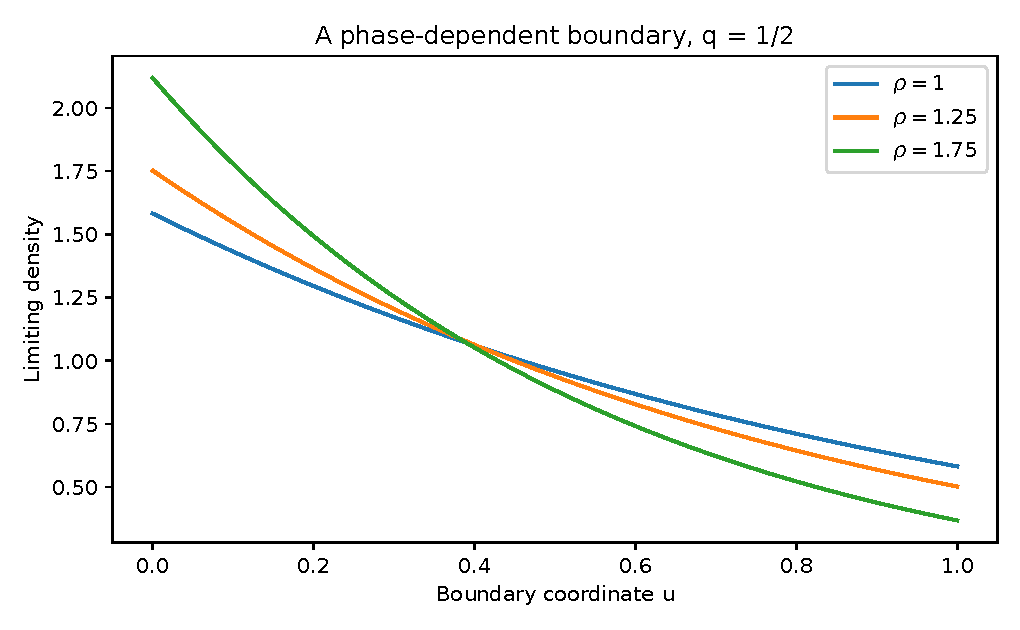
\includegraphics[width=.84\linewidth]{figures/boundary_phase.pdf}
\caption{The limiting density of $U_n$ for three geometric phases
when $q=1/2$. This is a phase effect in the \emph{conditional
configuration}, not an assertion that the scalar endpoint expansion
has a phase-free remainder.}
\label{fig:boundary}
\end{figure}

\section{A Brownian bridge inside a small Fabius event}
\label{sec:bridge}
Define a random continuous function $B_t$ by its grid values
\begin{equation}\label{eq:bridge-process}
 B_t(\ell/n)=\frac1{\sqrt n}\sum_{k=1}^{\ell}(Y_k-\mu(a_k)),
 \qquad \ell=0,\ldots,n,
\end{equation}
and interpolate linearly. Let $B^\circ$ be a standard Brownian
bridge: a centered continuous Gaussian process with covariance
$\Cov(B^\circ(s),B^\circ(u))=\min(s,u)-su$.

\begin{theorem}[Joint bridge and slack limit]\label{thm:bridge}
For geometric weights,
\begin{equation}\label{eq:bridge-limit}
 (B_t,D_t)\Rightarrow(B^\circ,E)
 \quad\hbox{in }C[0,1]\times\R,
\end{equation}
under $\Pt$, where $E\sim\Exp(1)$ is independent of $B^\circ$.
No subsequence restriction on the geometric phase is required.
\end{theorem}
\begin{proof}
\textit{Step 1: a product-law invariance principle.}
Couple the first $n$ tilted coordinates to independent exponentials
using independent uniforms $V_k$:
\[
 E_k=-\log(1-V_k),\qquad
 Y_k=-\log\bigl(1-(1-e^{-a_k})V_k\bigr).
\]
Then $Y_k\le E_k$ and
$\E(E_k-Y_k)=1-\mu(a_k)$. The proof of \cref{prop:active} gives
$\sum_{k\le n}(1-\mu(a_k))=O_q(1)$. Therefore the expected supremum
norm of the difference between $B_t$ and the linearly interpolated
centered exponential walk is at most $O_q(n^{-1/2})$.

For completeness, that exponential walk converges to Brownian
motion: independent increment central limit theorems give the
finite-dimensional limits, while
\[
 \E\left|\sum_{k=r+1}^{r+\ell}(E_k-1)\right|^4
 =\ell\E(E_1-1)^4+3\ell(\ell-1)=O(\ell^2)
\]
gives a useful fourth-moment bound. To check continuous-path
tightness explicitly, write an increment of the interpolated walk
as $n^{-1/2}\sum c_k(E_k-1)$, where $0\le c_k\le1$ and
$\sum c_k=n|v-u|$. Independence gives a fourth moment bounded by
$Cn^{-2}[(\sum c_k^2)^2+\sum c_k^4]$. If $|v-u|\ge1/n$, this
is at most $C'|v-u|^2$. If $|v-u|<1/n$, at most two coefficients
are nonzero and their sum is $n|v-u|$, giving the same bound.

For clarity, the resulting dyadic tightness argument is short.
Choose $0<\theta<1/4$. Markov's inequality and a union bound over
all $2^r$ adjacent dyadic increments at level $r$ bound the
probability that any exceeds $A2^{-\theta r}$ by
$CA^{-4}2^{-(1-4\theta)r}$. Summing over $r\ge R$ and chaining
dyadic approximations controls the modulus of continuity on
intervals of length $2^{-R}$ by a constant times
$A2^{-\theta R}$, outside a probability tending to zero uniformly
in $n$. This proves tightness. Thus under $Q_t$,
$B_t\Rightarrow B$, standard Brownian motion. The same coupling
and estimates apply to reversed blocks of the first $n$ coordinates.

\textit{Step 2: finite-dimensional conditional distributions.}
Fix $0<s_1<\cdots<s_r<1$ and put $\ell=\lfloor ns_r\rfloor$.
Choose $I=\{1,\ldots,\ell\}$. The complement has variance
$(1-s_r)n+O_q(1)$. By \cref{eq:joint-ratio,lem:ratio}, the joint
conditional law of the selected path values and $D_t$ is obtained,
up to a bounded likelihood-ratio error tending to zero in $L^1$,
by weighting the product law by
\begin{equation}\label{eq:bridge-weight}
 \frac1{\sqrt{1-s_r}}
       \exp\left(-\frac{B_t(s_r)^2}{2(1-s_r)}\right)
\end{equation}
and adjoining an independent exponential. The single next coordinate
may be included in $I$ without changing its limiting variance
fraction. The same bounded likelihood ratio then transfers the
vanishing interpolation error from $Q_t$ to $P_t$.

Under Brownian motion, \cref{eq:bridge-weight} is the likelihood
ratio for its restriction to $[0,s_r]$ when conditioned to have
value zero at time one. This can be checked directly: the density
of the independent remaining increment at $-B(s_r)$, divided by
the density of $B(1)$ at zero, is exactly the displayed expression.
Gaussian multiplication then gives covariance
$\min(s_i,s_j)-s_is_j$. The extra exponential variable stays
independent. This proves all interior finite-dimensional limits.

\textit{Step 3: tightness after conditioning.}
For any coordinate block with complement variance bounded below by
a positive fraction of $n$, \cref{eq:block-ratio} is uniformly
bounded. Apply this once to the first half of the active
coordinates, and once to the second half, read in reverse order.
Under $Q_t$ both centered half-paths are tight by Step 1. An event
with product probability $p$ has conditional probability at most
$Cp$ for each such half-path, so both modulus-of-continuity bounds
transfer to $P_t$. Combining the two bounds at the midpoint gives
tightness of $B_t$ on $[0,1]$; its value at the midpoint is tight
by the first-half bound.

To identify the endpoint, note that
\[
 \sqrt n B_t(1)=-D_t-Z_{\{k>n\}}.
\]
Here $|Z_{\{k>n\}}|\le\sum_{k>n}a_k=O_q(1)$ deterministically.
The slack is tight by \cref{thm:slack}; hence $B_t(1)\to0$ in
$P_t$-probability. Joint tightness with $D_t$ and the identified
finite-dimensional distributions prove \cref{eq:bridge-limit}.
\end{proof}

This describes two different scales simultaneously. Individual
strongly tilted contributions have size $t^{-1}$. A partial sum of
order $n$ such terms fluctuates on scale $\sqrt n/t$, while the
remaining distance to the inequality boundary is only of order
$t^{-1}$. Pinning the large-scale endpoint produces the bridge;
the one-sided microscopic gap produces the independent exponential.

\section{Beyond geometric decay}
\label{sec:other-weights}
The variance-fraction theorem is not tied to a functional equation
or to a dyadic product. It already applies to every positive summable
sequence. We calculate its variance clock for two other families,
illustrating why the abstract formulation is useful.

\subsection{Stretched-exponential weights}
\begin{proposition}\label{prop:stretched}
Let $w_k=e^{-ck^\beta}$ with $c,\beta>0$, and set
$N(t)=(\log t/c)^{1/\beta}$. Then
\[
 m(t)\sim N(t),\qquad V(t)\sim N(t),
\]
If $k(t)/N(t)\to\alpha\in[0,1]$ and
$I_t=\{1,\ldots,k(t)\}$, then $V_{I_t}/V(t)\to\alpha$.
Thus \cref{thm:main} gives the same profiles $\Delta(\alpha)$
and $K(\alpha)$ for these prefixes, including the endpoint
interpretations.
\end{proposition}
\begin{proof}
Fix $0<\varepsilon<1$. For $k\le(1-\varepsilon)N$,
\[
 a_k=\exp\{c(N^\beta-k^\beta)\}
 \ge\exp\{c[1-(1-\varepsilon)^\beta]N^\beta\}\to\infty
\]
uniformly. Their means and variances tend uniformly to one.
For $k\ge(1+\varepsilon)N$, the sums of $a_k$ and $a_k^2$
tend to zero. To see this explicitly, compare the decreasing
function $e^{-rcu^\beta}$ with its tail integral, for $r=1,2$.
After $z=rcu^\beta$, the integral is bounded by a polynomial in
$N$ times $e^{-rc(1+\varepsilon)^\beta N^\beta}$.
Multiplying by $t^r=e^{rcN^\beta}$ still leaves an exponentially
small bound. The intermediate indices are at most
$2\varepsilon N+O(1)$, each contributing at most one to either
mean or variance. Let $\varepsilon\downarrow0$ to obtain the
asymptotics.

The prefix assertion follows from the same three-region argument,
with an additional cut at $k(t)$.
\end{proof}

The geometric boundary theorem does not automatically extend in
its present form. The transition width in the coordinate index is
of order $N^{1-\beta}$ when this grows, rather than uniformly of
order one. A boundary scaling theorem for $\beta\ne1$ is therefore
a distinct question, not an unstated corollary.

\subsection{Polynomial weights}
\begin{proposition}\label{prop:polynomial}
Let $w_k=k^{-p}$ with $p>1$, and let $N=t^{1/p}$. Put
\begin{equation}\label{eq:CpDp}
 C_p=\int_0^\infty v(u^{-p})\,du,\qquad
 M_p=\int_0^\infty\mu(u^{-p})\,du.
\end{equation}
Both constants are finite and strictly positive, and
\begin{equation}\label{eq:polynomial-scales}
 V(t)\sim C_pN,\qquad m(t)\sim M_pN.
\end{equation}
For a prefix of length
$k(t)=\lfloor bN\rfloor$, $0<b<\infty$, its variance fraction tends
to
\begin{equation}\label{eq:poly-alpha}
 \alpha_p(b)=\frac{\int_0^b v(u^{-p})\,du}{C_p}\in(0,1).
\end{equation}
Its limiting total variation and relative entropy are respectively
$\Delta(\alpha_p(b))$ and $K(\alpha_p(b))$.
\end{proposition}
\begin{proof}
Here $a_k=(k/N)^{-p}$. The functions
$v(u^{-p})$ and $\mu(u^{-p})$ are continuous on $(0,\infty)$,
bounded at zero, and bounded at infinity by constants times
$u^{-2p}$ and $u^{-p}$ respectively. They are therefore integrable.
Riemann sums on $[\varepsilon,R]$ converge in the usual way. The
part $k<\varepsilon N$ contributes at most $\varepsilon N+1$;
the part $k>RN$ is bounded by convergent power tails. Let
$\varepsilon\downarrow0$, $R\to\infty$. This proves
\cref{eq:polynomial-scales} and the analogous truncated integral
for the prefix.

\end{proof}

\begin{remark}[A consistency relation between the two constants]
The identity $v(a)=\mu(a)-a\mu'(a)$ and integration by parts give
$C_p=(1-1/p)M_p$. Indeed, for $g(u)=\mu(u^{-p})$,
$v(u^{-p})=g(u)+(u/p)g'(u)$; the boundary term $ug(u)$ vanishes at
both endpoints because $p>1$. This agrees with differentiating
$x(t)\sim M_pt^{1/p-1}$ and the exact identity
$x'(t)=-V(t)/t^2$, but the integration proof avoids differentiating
an asymptotic equivalent without justification.
\end{remark}

\section{An exact lazy sampler and its expected cost}
\label{sec:sampling}
The original event $S_q\le x$ is rare, but after tilting the rejection
penalty is only of order $n^{-1/2}$. The infinite number of
coordinates must nevertheless be handled honestly.

\subsection{The ideal accept--reject identity}
A proposal from $Q_t$ has total $T=\sum Y_k=tS$. Accept it with
probability
\begin{equation}\label{eq:accept}
 A(T)=e^{T-m}\ind_{T\le m}.
\end{equation}
This is a valid probability in $[0,1]$. By \cref{eq:RN-full}, the
accepted distribution is exactly $P_t$ and the acceptance
probability is $J(t)$.

Each proposed coordinate can be generated from a scalar uniform
$V_k$ by
\begin{equation}\label{eq:inverse-cdf}
 Y_k=-\log\left(1-(1-e^{-a_k})V_k\right).
\end{equation}
Let $H$ be a separate uniform random variable used for acceptance.
For geometric weights, after the first $K$ coordinates have been
revealed,
\begin{equation}\label{eq:tail-interval}
 s_K=\sum_{k\le K}Y_k,\qquad
 r_K=\frac{tq^{K+1}}{1-q},\qquad T\in[s_K,s_K+r_K].
\end{equation}
The bound is deterministic, not a confidence interval.

\subsection{Lazy decision rule}
Start each proposal by generating the first $n$ coordinates and
$H$. Then apply the following rule, generating one additional
coordinate whenever the decision is unresolved.
\begin{lstlisting}
If s_K > m:
    reject.
Else if s_K + r_K <= m:
    If H <= exp(s_K - m):
        accept.
    Else if H > exp(s_K + r_K - m):
        reject.
    Else:
        reveal the next coordinate.
Else:
    reveal the next coordinate.
\end{lstlisting}
If accepted, the unrevealed coordinates remain available as a lazy
continuation. They are not falsely reported as a completed finite
representation of an infinite random sequence.

\begin{theorem}[Exactness and sampling complexity]\label{thm:sampler}
In a real-arithmetic model in which $q,t,m(t)$ and the operations in
\cref{eq:inverse-cdf} are exact, the lazy rule terminates almost
surely and its accepted infinite configuration has law $P_t$.
Let $K_t$ be the number of coordinate uniforms drawn for one
proposal, excluding $H$. For geometric weights,
\begin{equation}\label{eq:sampler-cost}
 \E K_t=n+O_q(n^{-1/2}),\qquad
 \E[\hbox{scalar uniform draws per accepted proposal}]
 \sim\sqrt{2\pi}\,n^{3/2}.
\end{equation}
The second count includes acceptance uniforms and all rejected
proposals; it excludes later requests for additional output
coordinates and the cost of precomputing $m(t)$.
\end{theorem}
\begin{proof}
Every decision follows from \cref{eq:tail-interval}
and agrees with the ideal rule $H\le A(T)$. If $T>m$, eventually
$s_K>m$. If $T<m$, eventually $s_K+r_K<m$, and the lower and upper
acceptance bounds tend to the common value $e^{T-m}$. The rule
therefore terminates unless $T=m$ or $H=e^{T-m}$. Both events have
probability zero: $T$ has a continuous distribution and $H$ is
independent and continuous. An accepted finite prefix is valid for
every continuation consistent with its bounds. Completing the
unrevealed proposal coordinates according to $Q_t$ therefore
recovers exactly the ideal accepted infinite law.

For the cost estimate, the first $n$ coordinates have variance
$n+O_q(1)$. Their centered sum has density bounded by $C_q/\sqrt n$
by \cref{thm:lclt}. Convolution with any additional independent
coordinates cannot increase this upper bound. Thus the uncentered
sum $s_K$, for every $K\ge n$, has density bounded by
$C_q/\sqrt n$.

A proposal unresolved after $K$ lies in one of two disjoint cases.
First, $s_K\le m<s_K+r_K$; its probability is at most
$C_qr_K/\sqrt n$. Second, $s_K+r_K\le m$ and $H$ lies strictly
between the two exponential acceptance bounds. Its probability is
at most
\begin{align*}
 \frac{C_q}{\sqrt n}\int_{-\infty}^{m-r_K}
   \bigl(e^{s+r_K-m}-e^{s-m}\bigr)\,ds
 &=\frac{C_q}{\sqrt n}(1-e^{-r_K})\\
 &\le\frac{C_qr_K}{\sqrt n}.
\end{align*}
Hence $\Pp(K_t>K)\le2C_qr_K/\sqrt n$ for $K\ge n$.
Since $r_K=\rho_tq^{K-n+1}/(1-q)$,
$\sum_{K\ge n}r_K=O_q(1)$. Summing the tail probabilities gives
the first assertion of \cref{eq:sampler-cost}.

Let $C_t=K_t+1$ count all scalar uniforms in a proposal. Success
has probability $J(t)$, independently across fresh proposal cycles.
Although cost and success within a cycle may be dependent, a
renewal identity gives expected total cost $\E C_t/J(t)$:
condition on the first cycle and restart after failure. Using
$J(t)\sim(2\pi V)^{-1/2}$ and $V\sim n$ proves the second
assertion.
\end{proof}

\begin{remark}[Exactness does not mean a proved bit-complexity bound]
The theorem counts exact-real coordinate draws. For computable
parameters and certified interval access to $m(t)$, the comparisons
can be refined until separated; the probability-zero equality
cases are the same as above. The series for $m$ has the explicit
mean-tail bound
$\sum_{k>K}\mu(tq^k)\le tq^{K+1}/[2(1-q)]$.
Nevertheless, arbitrary-precision transcendental evaluation and
random-bit costs have not been analyzed here. The accompanying
Python experiments use finite binary floating-point arithmetic and
a tail cutoff. They are \emph{not} that interval-certified exact
implementation.
\end{remark}

\section{Reproducible checks and numerical experiments}
\label{sec:experiments}
The package contains \texttt{code/verify\_conditioning.py}, CSV
outputs, numerical environment information, and the figure sources
in the form of the same reproducible script. No external dataset is
needed. All mathematical theorems above are proved independently
of this section.

\subsection{A finite-simplex model with exact formulas}
Let $Q^{(n)}$ be the law of $n$ independent rate-one exponentials,
and weight it by $e^{T-n}\ind_{T\le n}$, where $T$ is their sum.
The resulting $P^{(n)}$ is uniform on
\[
 \{(y_1,\ldots,y_n): y_i\ge0,\;\sum y_i\le n\}.
\]
This is an exactly solvable surrogate for the strongly tilted
active coordinates, not an equality with the geometric series.

For the first $k<n$ coordinates, put $s=\sum_{i\le k}y_i$. Their
likelihood ratio relative to $k$ independent exponentials is
\begin{equation}\label{eq:simplex-ratio}
 R_{n,k}(s)=\frac{n!}{(n-k)!n^k}\,e^s(1-s/n)^{n-k}\ind_{[0,n]}(s).
\end{equation}
Under $P^{(n)}$, $s/n$ has the $\operatorname{Beta}(k,n+1-k)$ law.
It follows that
\begin{align}\label{eq:simplex-kl}
 \KL(P^{(n)}_k\Vert Q^{(n)}_k)
 ={}&\log\Gamma(n+1)-\log\Gamma(n-k+1)-k\log n\notag\\
 &+\frac{nk}{n+1}
 +(n-k)\bigl[\psi(n-k+1)-\psi(n+1)\bigr],
\end{align}
where $\psi=(\log\Gamma)'$.

For total variation, $\log R_{n,k}(s)$ increases up to $s=k$ and
then decreases. Let $s_-\le k\le s_+$ be its two zeroes, with
$s_-=0$ for $k=1$. Then
\begin{equation}\label{eq:simplex-tv}
 \TV(P^{(n)}_k,Q^{(n)}_k)
 =P^{(n)}(s_-\le s\le s_+)-Q^{(n)}(s_-\le s\le s_+),
\end{equation}
which can be evaluated by beta and gamma distribution functions.
The formula follows by integrating the positive part of the
density difference, so there is no numerical optimization over
measurable sets.

\begin{table}[tb]
\centering\small
\begin{tabular}{rrrrr}
\toprule
$n$ & $k=n/2$ & TV & KL (nats) & Limiting TV / KL\\
\midrule
32 & 16 & 0.1652913 & 0.1052172 & $0.1660641\,/\,0.0965736$ \\
128 & 64 & 0.1658683 & 0.0988220 & $0.1660641\,/\,0.0965736$ \\
512 & 256 & 0.1660150 & 0.0971413 & $0.1660641\,/\,0.0965736$ \\
2048 & 1024 & 0.1660518 & 0.0967159 & $0.1660641\,/\,0.0965736$ \\
\bottomrule

\end{tabular}
\caption{The half-dimension finite-simplex comparison. The displayed
values evaluate exact formulas; numerical agreement does not itself
prove the infinite-series theorem.}
\label{tab:simplex}
\end{table}

\begin{figure}[tb]
\centering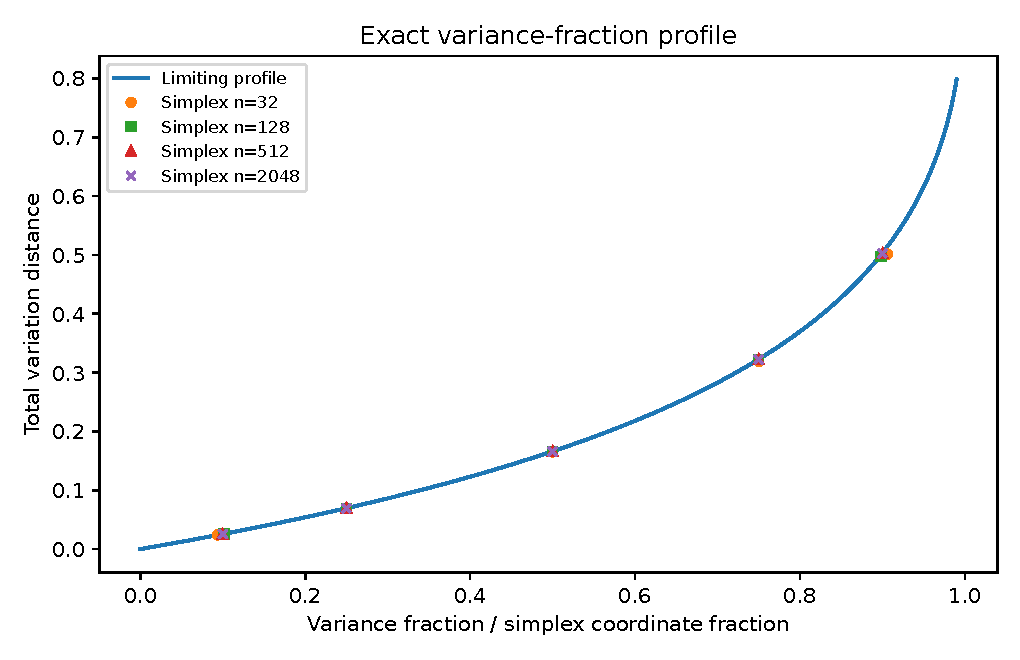
\includegraphics[width=.85\linewidth]{figures/tv_profile.pdf}
\caption{The exact limiting profile $\Delta$, with finite-simplex
values from \cref{eq:simplex-tv}.}
\label{fig:tv}
\end{figure}
\begin{figure}[tb]
\centering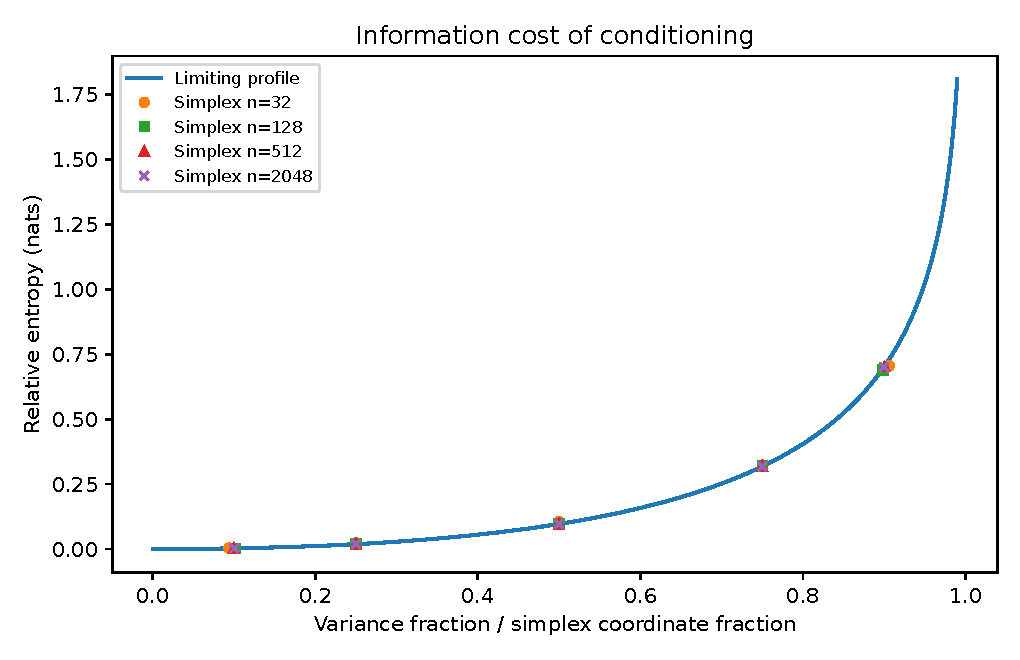
\includegraphics[width=.85\linewidth]{figures/kl_profile.pdf}
\caption{The relative-entropy profile $K$, with finite-simplex
values from \cref{eq:simplex-kl}.}
\label{fig:kl}
\end{figure}

\subsection{Algebraic and quadrature checks}
The script checks the normalization and mean of the truncated
exponential, the identity $v=\mu-a\mu'$, and the Taylor coefficients
through degree six. It also checks 72 exact polynomial integrals:
normalization and first moments for every simplex marginal with
$2\le n\le9$ and $1\le k<n$.

Four selected simplex cases are evaluated independently by
one-dimensional quadrature. In the delivered run, the maximum
absolute discrepancy was below $1.4\times10^{-15}$ for total
variation and $3.0\times10^{-13}$ for relative entropy. Stable
mean/variance formulas were compared to quadrature over nine
widths from $10^{-5}$ to $60$, with maximum absolute discrepancy
below $2.3\times10^{-16}$. These are numerical residuals, not
interval-certified error bounds.

\subsection{Direct geometric-series experiments}
For $q=1/2$, $\rho=1.25$, and $n=32,128,512$, the script generated
160,000 tilted proposals at each dimension using a fixed documented
seed. It retained proposals according to the floating-point
version of \cref{eq:accept}. The scaled sum of all omitted support
widths was below $2\times10^{-13}$. This controls deterministic
series truncation, not rounding error or the difference between the
finite experiment and a certified sampler.

\begin{table}[tb]
\centering\small
\begin{tabular}{rrrrrr}
\toprule
$n$ & Accepted & $\widehat{\E D}$ & SE &
 $\widehat{\Var B(1/2)}$ & $\widehat{\E U_n}$\\
\midrule
32 & 11,458 & 0.9699 & 0.0089 & 0.2240 & 0.4008 \\
128 & 5,733 & 0.9965 & 0.0130 & 0.2511 & 0.4025 \\
512 & 2,733 & 1.0364 & 0.0203 & 0.2507 & 0.3919 \\
\bottomrule

\end{tabular}
\caption{Direct tilted-proposal experiments. Limits are $1$ for
$\E D$, $1/4$ for the midpoint bridge variance, and
$1/1.25-1/(e^{1.25}-1)\approx0.398449$ for $\E U_n$.
SE is the empirical standard error of the slack mean. Finite-size
bias and sampling fluctuations remain visible.}
\label{tab:geometric}
\end{table}

\begin{figure}[tb]
\centering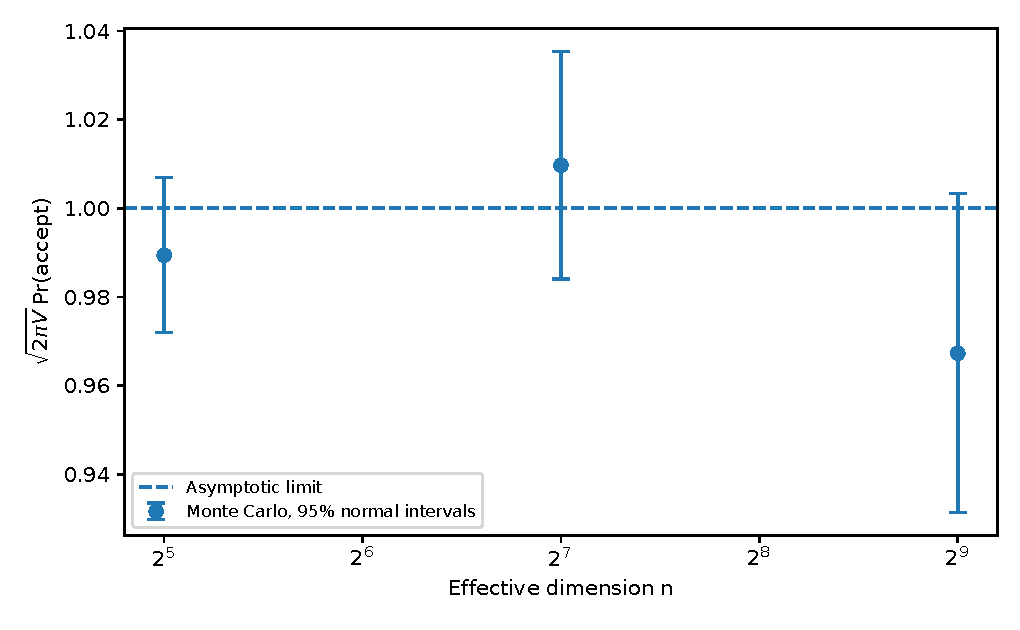
\includegraphics[width=.85\linewidth]{figures/acceptance.pdf}
\caption{Normalized acceptance probabilities. Bars show approximate
95\% normal sampling intervals, not certified enclosures. The
predicted limit is one.}
\label{fig:acceptance}
\end{figure}

The experiment at $n=512$ accepted fewer than three thousand
configurations, so it should not be read as a high-precision check
of all observables. In particular a slack mean above one in that
run is compatible with sampling error. The proof establishes the
limit; the experiment checks the normalization, indexing, and
plausibility of the finite-dimensional formulas.

\section{Further research questions and a concrete development plan}
\label{sec:future}
The results identify a structure worth extending, rather than
closing every issue about conditional Fabius laws. The following
questions are proposed research directions, not additional theorems.

\subsection{Quantitative and critical-regime questions}
\begin{question}[Uniform finite-$t$ errors]\label{q:rates}
Can one give explicit bounds for the difference between the block
likelihood ratio and \cref{eq:h-approx}, uniform for
$\alpha_t\le1-\varepsilon_t$ when $\varepsilon_t\downarrow0$?
\end{question}
The current proof fixes a positive complement fraction. A useful
next target is a bound expressed in the complement variance and
its third and fourth cumulants. This would make the threshold
usable as a certified finite-precision rule, rather than solely
an asymptotic classification.

\begin{question}[The critical complement]\label{q:critical}
What replaces the Gaussian profile when $V_J$ stays bounded,
or tends to infinity much more slowly than $V$?
\end{question}
For geometric weights and a block ending within $O(1)$ of $n$,
the complement has the phase-dependent law of
\cref{thm:boundary}. Inserting its actual density into
\cref{eq:block-ratio} is a plausible route to a matched
macroscopic-to-boundary formula. The theorem that TV tends to one
at fraction one does not determine that finer rate.
% ed. (2026-09-30): two later packages answer this question for geometric weights
\begin{ednote}
Two independently written packages beside this one answer this question
for geometric weights, for different unobserved coordinates; neither cites
the other. \path{../Critical_Complements_Fabius_Conditioning/} (batch~66 of
the repository's \path{docs/incoming/}) hides a fixed number $r$ of early
coordinates together with the tail and proves
$\sqrt{2\pi n}\,(1-\TV)=\Lambda_n+r\log\Lambda_n+\log K-\log(r!)+1+o(1)$,
$\Lambda_n=\frac12\log(2\pi n)$, with the divergences of every fixed
R\'enyi order and an order-zero R\'enyi crossover; a growing number of
hidden early coordinates stays open there.
\path{../Critical_Complements_Sharp_Information_Loss/} (batch~68) follows
the route suggested above: it observes $\{1,\ldots,n-m\}$ and hides the
last $m$ coordinates before the boundary together with the tail, with the
boundary law of \cref{thm:boundary}. For fixed $m$ it gives a two-term
overlap expansion with an explicit phase constant and the relative entropy
to order $1/n$; for every $m=o(n)$ it gives the leading overlap through the
two real branches of Lambert~$W$, with a change of regime at
$m\asymp\log n$, and relative entropy $\frac12\log(n/m)-\frac12+o(1)$ when
$m\to\infty$. The two coincide only when nothing but the tail is hidden,
where their corrected overlap theorems agree after the phase change
$\rho\mapsto\rho/q$ (the first package's $\log K=0.486134172\ldots$ at
$q=1/2$, $\rho=1$ is the second's constant $K_{1/2,1/2,0}$). For a bounded hidden
complement both leading overlap terms agree with \cref{eq:overlap}, and the second package's
full-configuration entropy re-proves \cref{eq:full-kl} for geometric weights.
General weights and \cref{q:edgeworth} are not treated.
\end{ednote}

\begin{question}[Phase-sensitive higher corrections]\label{q:edgeworth}
Can the repository's all-orders scalar saddle expansions be
combined with \cref{eq:joint-ratio} to obtain conditional Edgeworth
expansions, including the geometric phase and the slack variable?
\end{question}
This would connect the present configuration-level results directly
to the existing exact-phase endpoint machinery. Uniform remainder
control in the selected block sum, not just formal Gaussian
integration, is the principal analytic obligation.

\subsection{Generality and structural extensions}
\begin{question}[Quantitative shape-based local limits]\label{q:shape}
Can the weak-to-uniform upgrade in \cref{lem:shape} be made
quantitative with a useful universal modulus, and then combined
with a Berry--Esseen bound to give explicit conditional error
bounds for arbitrary positive summable weights?
\end{question}
The qualitative regularity question is settled here: no weight
spacing or nonconcentration assumption is needed. The next issue
is effectiveness. The proof near the mode uses both monotonicity
and a log-concave midpoint inequality; optimizing that argument
may yield a universal, though not necessarily optimal, rate.

\begin{question}[Several simultaneous constraints]\label{q:multi}
For vector sums $\sum w_k^{(r)}U_k$ constrained near a boundary
point, is the block information profile governed by a covariance
fraction matrix, with a determinant analogue of $K(\alpha)$?
\end{question}
The scalar Gaussian calculation suggests an expression involving
$-\log\det(I-A)-\operatorname{tr}A$, but feasibility cones and
multiple slack coordinates change the local geometry. This
expression is a heuristic target, not a proved multivariate result.

\begin{question}[Other endpoint densities and random environments]
If the coordinate density behaves as $u^{\gamma-1}$ near zero,
can one replace exponentials by gamma limits and obtain the same
variance-based profile? For random weights, which quenched
hypotheses preserve it, and how does the boundary phase become
random?
\end{question}
A proof would need uniform moment and characteristic-function
bounds for the new tilted family, together with a precise
nonconcentration condition. Merely replacing a density in the
final formulas is not enough.

\begin{question}[Nongeometric boundary fields]
What is the limiting transition process for
$w_k=e^{-ck^\beta}$, $\beta\ne1$, and for $w_k=k^{-p}$?
\end{question}
The geometric boundary is a countable product indexed by an
$O(1)$ window. A growing transition window suggests a field or a
variance-time process rather than the same fixed-index limit.
The polynomial fraction $\alpha_p(b)$ supplies a natural clock.

\subsection{Algorithms and formal proof}
\begin{question}[Certified random-bit complexity]
Can a computable version of the lazy sampler be implemented with
interval arithmetic, with proved expected random-bit and
arithmetic costs at a requested endpoint precision?
\end{question}
A sensible implementation order is: stable enclosures for
$\mu,v$; certified bounds on $m$ and the geometric tail; a
random-bit inverse-CDF primitive; and a terminating comparison
loop with a measured precision distribution. Optimality among
adaptive proposals is a separate question: \cref{thm:sampler}
proves a cost, not a lower bound on all samplers.

For Lean integration, the most reusable milestones are the
truncated-exponential moment identities, the exact scalar
likelihood-ratio identity, the abstract local-limit-to-conditioning
transfer lemma, and the finite Gaussian integrals producing
$\Delta$ and $K$. The shape-based local central limit theorem and the
functional tightness argument should be separate modules with
explicit hypotheses. Numerical tables must stay outside the
trusted proof boundary unless connected by a verified checker,
consistent with the repository's stated architecture \cite{repo}.

\section{Conclusion}
The passage from endpoint probabilities to conditioned
configurations reveals an exact boundary for product behavior.
A block is asymptotically independent of the rare-event constraint
precisely when it uses a negligible share of the tilted variance.
At a positive fraction, its full discrepancy is captured by one
Gaussian variance reduction, producing explicit total-variation
and entropy profiles. At fraction one the two laws separate.

In the Fabius and geometric cases, that bulk statement coexists
with an infinite phase-sensitive transition law, Brownian-bridge
partial sums, and independent exponential slack. The same local
limit mechanism also yields a lazy exact-real sampler with a
polynomial expected draw count in the effective dimension. These
are proof-level extensions of the scalar endpoint viewpoint,
with quantitative rates, critical complements, and certified bit
complexity left as well-defined further problems.

\appendix
\section{Additional details for the finite-simplex formulas}
\label{app:simplex}
The volume of the positive simplex
$\{y\in\R_+^n:\sum y_i\le n\}$ is $n^n/n!$, so its uniform
density is $n!/n^n$. Integrating out $n-k$ coordinates leaves
\[
 p_k(y_1,\ldots,y_k)
 =\frac{n!}{n^n(n-k)!}(n-s)^{n-k}\ind_{s\le n}.
\]
Dividing by $e^{-s}$ gives \cref{eq:simplex-ratio}.
The sum of $k$ nonnegative coordinates has cross-sectional factor
$s^{k-1}/(k-1)!$, hence density
\[
 \frac{n!}{(k-1)!(n-k)!n^n}s^{k-1}(n-s)^{n-k},\qquad0<s<n.
\]
This is the scaled beta density claimed in
\cref{sec:experiments}. The beta integral and its derivative give
\[
 \E s=\frac{nk}{n+1},\qquad
 \E\log(1-s/n)=\psi(n+1-k)-\psi(n+1),
\]
which prove \cref{eq:simplex-kl}. Finally
\[
 \frac{d}{ds}\log R_{n,k}(s)=1-\frac{n-k}{n-s}
 =\frac{k-s}{n-s}.
\]
For $k>1$, $R_{n,k}(0)=\prod_{j=0}^{k-1}(1-j/n)<1$;
at its maximum it must exceed one because it integrates to one
under $Q_k$ and is not constant. Thus it has exactly the two
crossings used in \cref{eq:simplex-tv}. For $k=1$, the lower
crossing is zero. These facts justify the root brackets in the
numerical script.

The finite model also reproduces the profile by elementary
asymptotics. Under the product law,
$(s-k)/\sqrt k\Rightarrow N(0,1)$. Taylor expansion of
$\log R_{n,k}(s)$ around $s=k$ and Stirling's formula, for
$k/n\to\alpha\in(0,1)$, give
\[
 \log R_{n,k}(s)
 =-\tfrac12\log(1-\alpha)
   -\frac{\alpha}{2(1-\alpha)}\left(\frac{s-k}{\sqrt k}\right)^2
   +o(1)
\]
on central windows. This is the same $r_\alpha$ as in
\cref{eq:r-alpha}; the infinite-series proof supplies the missing
uniform likelihood-ratio control directly, rather than inferring
it from this finite analogy.

\section{Proof dependency and repository integration audit}
\label{app:audit}
\begin{center}\small
\begin{tabularx}{\linewidth}{@{}p{.25\linewidth}Xp{.22\linewidth}@{}}
\toprule
Result & Main inputs & Status in this package\\
\midrule
Tilt and moment formulas & Product integration, bounded differentiation & Proved here\\
Subset density theorem & Uniform moments, log-concavity, shape convergence & Proved here\\
Slack and full entropy & Density theorem, exact change of measure & Proved here\\
Sharp block profiles & Complement density, Gaussian integrals & Proved here\\
Geometric boundary & Subcritical-block theorem, product continuity & Proved here\\
Brownian bridge & Product invariance principle, bounded density ratios & Proved here\\
Other weight families & Riemann sums and elementary tail estimates & Proved here\\
Lazy sampler & Exact acceptance identity, geometric tail bounds & Proved in stated model\\
Python diagnostics & Symbolic checks and floating-point calculations & Executed, not formal proofs\\
Lean declarations & None supplied or compiled for these new results & Not claimed\\
\bottomrule
\end{tabularx}
\end{center}

The repository was consulted at commit
\nolinkurl{e2b1f016a94102663f12b970e6dd434229f90d01}. The principal
specific source read was
\begin{quote}\small\ttfamily
Analysis/FabiusFunction/Lean/FabiusFunction/\allowbreak
PaperFabiusAsymptotic.lean
\end{quote}
whose blob is
\nolinkurl{d9508bee558197a19a90b615f9ee84e29ee3b793}.
Its claim-level audit explains the status of the scalar endpoint
expansions. The frontier README and draft manifest were also
consulted to understand the mixed formalized/prose research
boundary. This was a targeted source inspection, not a repository
build or an exhaustive claim-by-claim comparison with its entire
research corpus.

No theorem above is labeled Lean-verified merely because nearby
scalar results have Lean counterparts. Conversely, the proofs here
do not assume the correctness of every claim in the repository.
All distributional assertions needed for the new theorem package
are established in this article from the displayed random-series
model with positive summable weights.

\section{Reproduction instructions and artifact scope}
The source file \texttt{article.tex} compiles with pdfLaTeX and
standard TeX Live packages, including Libertinus. The figures and
two table fragments are included in the package, so rebuilding the
PDF does not require rerunning Monte Carlo.
\begin{lstlisting}[language=bash]
pdflatex -interaction=nonstopmode -halt-on-error article.tex
pdflatex -interaction=nonstopmode -halt-on-error article.tex
pdflatex -interaction=nonstopmode -halt-on-error article.tex
\end{lstlisting}
To rerun the diagnostic suite and regenerate the data and figures:
\begin{lstlisting}[language=bash]
python -m pip install -r requirements.txt
python code/verify_conditioning.py --proposals 160000
python code/make_tables.py
\end{lstlisting}
The first command is optional when dependencies are already
installed. The environment used for the delivered run is recorded
in \texttt{data/environment.json}. The script uses a documented
fixed pseudorandom seed; exact byte-for-byte agreement of plots
across library versions is not promised. No font files are included.

\begin{thebibliography}{99}
\bibitem{fabius}
J. Fabius,
\emph{A probabilistic example of a nowhere analytic
$C^\infty$-function},
Zeitschrift f\"ur Wahrscheinlichkeitstheorie und Verwandte Gebiete
\textbf{5} (1966), 173--174.
\href{https://doi.org/10.1007/BF00536652}{doi:10.1007/BF00536652}.

\bibitem{arias}
J. Arias de Reyna,
\emph{An infinitely differentiable function with compact support:
Definition and properties},
arXiv:1702.05442 (2017), English translation of the 1982 article.
\url{https://arxiv.org/abs/1702.05442}.

\bibitem{diaconisfreedman}
P. Diaconis and D. A. Freedman,
\emph{Conditional limit theorems for exponential families and finite
versions of de Finetti's theorem},
Journal of Theoretical Probability \textbf{1} (1988), 381--410.
\href{https://doi.org/10.1007/BF01048727}{doi:10.1007/BF01048727}.

\bibitem{dembozeitouni}
A. Dembo and O. Zeitouni,
\emph{Refinements of the Gibbs conditioning principle},
Probability Theory and Related Fields \textbf{104} (1996), 1--14.
\href{https://doi.org/10.1007/BF01303799}{doi:10.1007/BF01303799}.

\bibitem{catorferrari}
E. Cator and P. A. Ferrari,
\emph{Gibbs conditioning principle for log-concave independent
random variables}, arXiv:2512.24910v2, 21 April 2026.
\url{https://arxiv.org/abs/2512.24910v2}.
The cited comparison is to the explicit integer-valued setup in
this version.

\bibitem{prekopa}
A. Pr\'ekopa,
\emph{On logarithmic concave measures and functions},
Acta Scientiarum Mathematicarum (Szeged) \textbf{34} (1973),
335--343. The one-dimensional convolution argument used here is
reproved in \cref{lem:logconcave}.

\bibitem{repo}
V. Reshetnikov and contributors,
\emph{ProveIt}, repository snapshot
\nolinkurl{e2b1f016a94102663f12b970e6dd434229f90d01},
consulted 28 September 2026 (Pacific time).
\url{https://github.com/VladimirReshetnikov/ProveIt/tree/e2b1f016a94102663f12b970e6dd434229f90d01}.
In particular, the Fabius endpoint claim audit at
\nolinkurl{Analysis/FabiusFunction/Lean/FabiusFunction/PaperFabiusAsymptotic.lean}.
\end{thebibliography}
\end{document}
